%\section{Ist-Zustand}
%Das aktuelle System ist eine prototypische Weiterentwicklung der :em ALM. Das Projekt ist eine Weiterentwicklung der auf Atlassian Tools basierenden Application Lifecycle Managment (ALM) Umgebung, die in der DMZ der :em AG gehostet wird. Diese beinhaltet zurzeit die manuell installierten Atlassian Tools Jira, Confluence, Bitbucket und Crowd auf einzelnen VMs. Im Gegensatz dazu werden Anwendungen in der :em ALM v2 in einem Kubernetes Cluster bereitgestellt. Dafür wurden basierend auf bereits existierenden Containern der Atlassian Tools Helm Charts erstellt. Dieser Helm Chart enthält neben der Anwendung selbst und einer Datenbank auch einen Container, welcher ein Script für die Initiale Einrichtung über den Setup-Wizard, sowie die anschließende Konfiguration vornimmt. So ist es möglich innerhalb einer kurzen Zeit bei Bedarf eine für Instanz einer Anwendung bereitzustellen. Dadurch ist es nicht mehr nötig mehrere Bereiche innerhalb einer Anwendung für verschiedene Kunden zu erstellen, sondern für jeden kann eine eigene bereitgestellt werden.
%Die :em AG ist offizieller Atlassian Silver Solution Partner und bietet u. A. verschiedene Dienstleistungen rund um Atlassian Produkte an. Die ":em ALM" ist eine auf Atlassian Tools basierte ALM (Application Lifecycle Management) Umgebung die durch die :em AG zur Zusammenarbeit mit Kunden auf eigener Hardware :em DMZ gehostet wird. Aktuell beinhaltet sie die manuell installierten Atlassian Tools JIRA, Confluence, Bitbucket und Crowd auf einzelnen VMs. Seitens unserer Kunden ist verstärktes Interesse an Containerlösungen und DevOps Ansätzen zu beobachten. Aus diesem Grund besteht der Inhalt dieser Bachelorarbeit in der vollautomatisierten Bereitstellung unserer eigenen ALM Umgebung mit Containern. Eine prototypische Realisierung, die im Rahmen einer Studienarbeit entstanden ist bereits vorhanden. Die Praxisphase + Bachelorarbeit beinhaltet die Fertigstellung der prototypischen Realisierung und folgende zusätzliche Aspekte (Teilmenge möglich)

\chapter{Implementierung}
\label{cha:implementierung}
Das vorherige Kapitel widmete sich der Evaluation der in Kubernetes existierenden Persistenzlösungen. Dafür wurden die in der Kubernetes Dokumentation genannten Volume Plugins anhand der vorher aufgestellten Anforderungen bewertet und basierend auf dieser eine Handlungsempfehlung gegeben. In diesem Abschnitt wird die Umsetzung der Handlungsempfehlung für das aktuelle System geplant und ausgeführt. Abschließend wird die finale Umsetzung betrachtet und ein Fazit erarbeitet.

\section{Ist-Zustand}
Die Abbildung \ref{fig:clusteralt} zeigt den aktuellen Aufbau des Kubernetes Cluster der prototypischen Umsetzung der ALM v2.0 (siehe \ref{projekt}). Dieses besteht, um eine möglichst hohe Trennung der Anwendungen selbst von der Verwaltung zu erreichen, aus vier virtuellen Maschinen, wobei zwei davon als Worker Nodes (siehe \ref{workernode}) die eigentlichen Pods der Anwendungen ausführen. Die zwei Worker Nodes verfügen mit je 24 Gigabyte Arbeitsspeicher und sechs Prozessorkernen über eine wesentlich bessere Ausstattung als die zwei Master Nodes (siehe \ref{masternode}) mit vier Prozessorkernen und vier Gigabyte Arbeitsspeicher.
%In einer vorherigen Version der Umsetzung bestand das Cluster aus drei Nodes auf virtuellen Maschinen, welche alle Rollen zugeteilt bekamen.
%evlt warum der wechsel
\begin{figure}[htb]
\centering
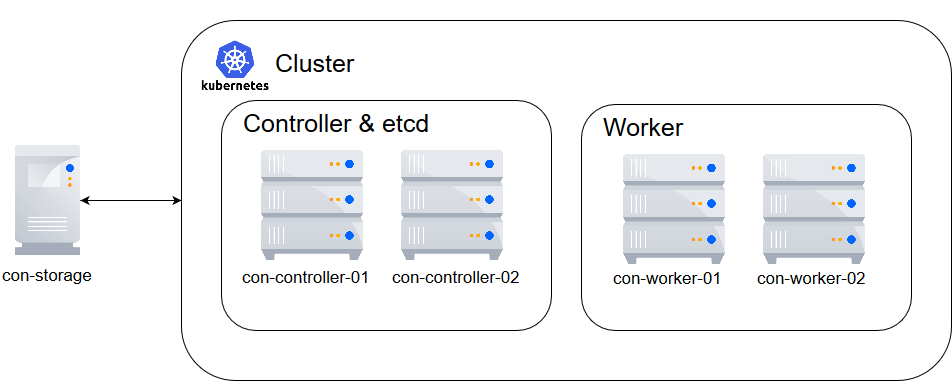
\includegraphics[width=1\textwidth,angle=0]{gfx/cluster_alt.png}
\caption[Cluster: Aktuelle Architektur]{Cluster: Aktuelle Architektur}
\label{fig:clusteralt}
\end{figure}
Um den Zustand und die Daten der Anwendungen zu speichern, wurde zuerst eine auf einem Blockspeicher basierende Speicherlösung eingesetzt, welche direkt im Kubernetes Cluster lief. Im Laufe des Projekts wurde diese, da sie kein \ac{RWX} unterstützt, durch einen zentralen NFS Server ersetzt. Diese virtuelle Maschine ist nicht redundant ausgelegt, befindet sich aber innerhalb einer Backup-Routine, welche täglich eine Sicherung des Systems erstellt. Die Datenträger für die Pods werden dynamisch durch den \textit{nfs-client-provisioner} (siehe \ref{eva:nfskube}) erzeugt, wobei die Konfiguration dieser über die Parameter der Helm Charts erfolgt.

\section{Planung}
\label{sec:planung}
Während der Planung der Integration von GlusterFS in das Kubernetes Cluster stellt sich zunächst die zentrale Frage, ob die Persistenzlösung innerhalb des Kubernetes Clusters oder als eigenständiges Speichercluster agieren soll. Während die Integration innerhalb des Kubernetes Clusters Vorteile wie eine schnelle Installation und eine gute Skalierbarkeit mit sich bringt, hilft das Aufsetzen außerhalb des Clusters dabei eine bessere Trennung zu schaffen. Da sich das Projekt im ständigen Wandel befindet und dies ebenfalls das Kubernetes Cluster betrifft, soll das GlusterFS-Cluster möglichst unabhängig agieren. Für die Installation stehen mehrere Hilfsmittel bereit. Neben der offiziellen Dokumentation bietet Gluster auch Skripte für die automatische Installation über Ansible, einem Tool für das automatische Aufsetzen und Konfigurieren von Systemen. \medskip

Durch das Aufbauen eines Speicherclusters verändert sich die Architektur des Clusters. Dabei wird der vorher für die Speicherung zuständige zentrale NFS-Server durch ein GlusterFS Cluster ersetzt. Für dieses werden drei virtuelle Maschinen erstellt, welche im Verbund für die Speicherung zuständig sind. Durch das Verwenden von drei Servern ist es möglich, durch eine dreifache Redundanz die Chance auf einen Split-Brain Zustand gering zu halten.
%evtl 3 Replicas wegen Split brain
\begin{figure}[htb]
\centering
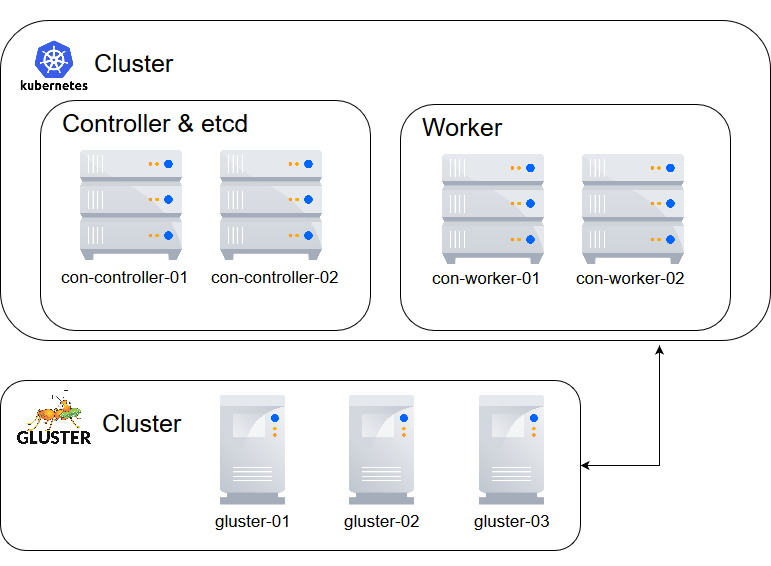
\includegraphics[width=1\textwidth,angle=0]{gfx/cluster_neu.png}
\caption[Cluster: Neue Architektur]{Cluster: Neue Architektur}
\label{fig:clusterneu}
\end{figure}
Die Abbildung \ref{fig:clusterneu} zeigt den geplanten zukünftigen Aufbau des Systems. Während am Kubernetes Cluster keine Änderung durchgeführt wurde, wurde der NFS Server durch ein Speichercluster aus drei Systemen ersetzt. Dieses agiert als eigenes Cluster und kann so auch unabhängig vom Kubernetes Cluster betrieben und auch in anderen Projekten verwendet werden. 


\section{Umsetzung}
Die Integration von GlusterFS in das Kubernetes Cluster besteht aus zwei Schritten. Sie beginnt mit dem Aufsetzen der virtuellen Maschinen und der Installation und Konfiguration des Speicherclusters. Sobald dieses eigenständige System funktional ist, beginnt mit der Integration in das Kubernetes Cluster und dem Einrichten für die dynamische Datenträgererstellung der zweite Schritt.

\subsection{Installation und Konfiguration von GlusterFS}
Die Umsetzung beginnt mit dem Erzeugen drei neuer virtueller Maschinen. Diese erhalten jeweils ein Gigabyte Arbeitsspeicher, zwei Prozessorkerne sowie zwei Festplatten. Die Erste ist dabei für die Linux-Distribution Debian und die Daten des Betriebssystems zuständig während auf der Zweiten die Daten von GlusterFS abgelegt werden.
Um die Installation und Konfiguration möglichst einfach zu halten, wird dies aus einer Kombination von mehreren Skripten für Ansible umgesetzt. Für die Installation unter Debian wird die von Jeff Geerling auf Github veröffentlichte Rolle für Ansible genutzt \cite{gluster:ansibledebian}. \medskip

Ist die Installation abgeschlossen, wird die Konfiguration über die von Gluster veröffentlichten Ansible Rollen \cite{gluster:ansible} vorgenommen. Diese enthalten unterschiedliche Rollen für Wartung, die Aktivierung von Funktionen, das Aufsetzen und Verwalten des Clusters und das Erstellen und Verwalten von Datenträgern.
Für die Konfiguration müssen unter Nutzung der Rolle \textit{gluster.infra} zuerst die Datenträger erstellt und anschließend diese und das Speichercluster durch \textit{gluster.cluster} konfiguriert werden. Werden hier bereits virtuelle Datenträger für die Verwendung im Kubernetes Cluster oder in einem anderen Projekt erstellt, bieten die Parameter die Möglichkeit, die Anzahl an Redundanzen und weitere Einstellungen zu konfigurieren. \medskip

Abschließend werden die neuen Systeme noch in eine Backup-Routine integriert. Dafür wird das Skript, welches bereits beim zentralen NFS Server genutzt wurde, erneut verwendet. 


\subsection{Einbinden von GlusterFS in Kubernetes}
Nachdem das Speichercluster installiert wurde, kann es im Kubernetes Cluster für die dynamische Erstellung von Datenträgern eingerichtet werden. Eine Möglichkeit wäre das Einbinden eines zuvor erstellten virtuellen Datenträgers durch den bereits verwendeten \textit{nfs-client-provisioner}. Dies würde bedeuten, dass alle gespeicherten Daten in getrennten Verzeichnissen auf diesem Datenträger erzeugt werden. \medskip


Um für jede Anwendung automatisch einen virtuellen Datenträger in GlusterFS erstellen zu lassen, welcher an die Nutzer der Anwendung ausgehändigt werden kann, wird Heketi benötigt. Heketi ist eine Software, welche eine \ac{REST} Schnittstelle für das Erzeugen und Verwalten von GlusterFS-Datenträgern bietet. \medskip

Um diese Anwendung zu installieren, sind einige Schritte notwendig \cite{gluster:includekubernetesteps}. Um diese Schritte zu automatisieren, hat Gluster ein Skript veröffentlicht \cite{gluster:includekubernete}. Durch dieses wird Heketi im Kubernetes Cluster bereitgestellt und die Kommunikation mit dem Speichercluster sichergestellt. Damit Heketi einwandfrei funktioniert, wird noch eine passende \textit{topology.json} benötigt. In dieser Datei werden, damit Heketi die Architektur des Speicherclusters kennt, die einzelnen Nodes des GlusterFS Systems, sowie ihr Hostname, ihre IP-Adresse und ihre Datenträger definiert.

\section{Fazit}
Der Wechsel von einem zentralen NFS Server als Speicherlösung auf ein GlusterFS Cluster war durch die verfügbaren Skripte einfach möglich. Auch bieten diese Skripte Funktionen für die Verwaltung und Wartung des Clusters wie zum Beispiel die Skalierung und das manuelle Erstellen von Datenträgern. \medskip

Die Verwendung im Kubernetes Cluster gestaltet sich durch die Verwendung von Heketi ebenfalls einfach. Wie auch zuvor bei dem NFS Server ist es nach der Integration im Kubernetes Cluster möglich, ohne die unterliegende Architektur des Speichers zu bemerken, Datenträger dynamisch erstellen zu lassen. Diese können anschließend bei Bedarf durch Dritte eingebunden und modifiziert werden.
% MEHR MEHR MEHR - Eigene Erfahrungen